\section{Die \texorpdfstring{$\color{darkred}\SI{21}{\centi\meter}$}{21 cm}-Linie}
\subsection{Geschichte}
\begin{frame}{Geschichte}%
  \begin{columns}[c, onlytextwidth]%
    \column{0.15\textwidth}%
      \centering
      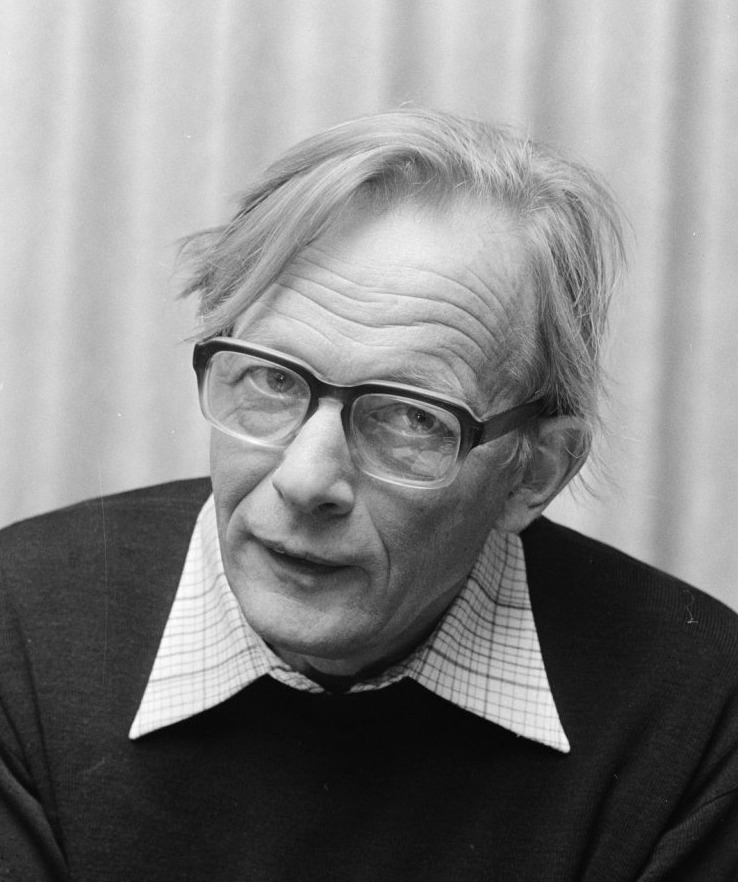
\includegraphics[width=\linewidth]{./images/Hendrik_vanDeHulst.jpg}
      \newline H. v.\,d. Hulst
    \column{0.8\textwidth}%
      \begin{description}[Hendrik van de Hulst]
        \item[Hendrik van de Hulst] Holländischer Astronom \& Mathematiker
        \item[1944] Vorhersage der \SI{21}{\centi\meter}-Linie
        \item[später] Mitarbeit bei der Kartographie der Milchstraße
      \end{description}
  \end{columns}%
  \vfill
  \begin{columns}[c, onlytextwidth]%
    \column{0.15\textwidth}%
      \centering
      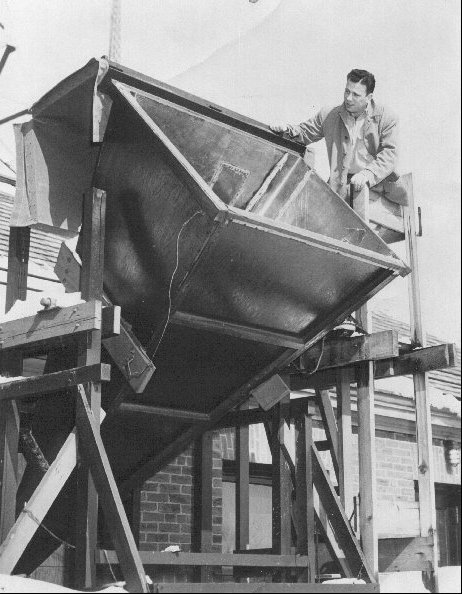
\includegraphics[width=\linewidth]{./images/ewenhorn.jpg}%
      \newline H.~Ewen
    \column{0.65\textwidth}%
      \begin{description}[1951]
        \item[1951] Entdeckung durch Edward Purcell \& Harold Ewen\\
                    an der Harvard University
      \end{description}
    \column{0.15\textwidth}%
      \centering
      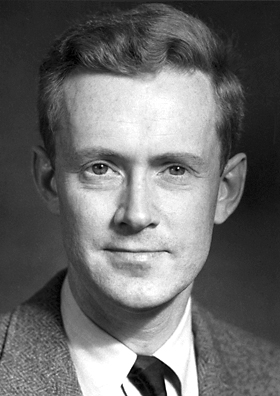
\includegraphics[width=\linewidth]{./images/Edward_Mills_Purcell.jpg}%
      \newline E.~Purcell
  \end{columns}%
\end{frame}
\subsection{Entstehung}
\begin{frame}{Die \SI{21}{\centi\meter}-Linie}
  \begin{columns}[c, onlytextwidth]%
    \begin{column}{0.6\textwidth}%
      \begin{tikzpicture}[
    level/.style={very thick},
  photon/.style={-{Stealth[length=2mm]}, thick, decorate, decoration={snake, pre length=1mm, post length=2mm,}}, connect/.style={dashed, very thick},
  ]
  \draw[level] (0, 0) -- (+1.5, 0) node at (0, 0) [above] {$1^2S_{\sfrac{1}{2}}$};
  \draw[connect] (1.5, 0) -- +(1.5,  1);
  \draw[connect] (1.5, 0) -- +(1.5, -1);
  \draw[level] (3,  1) -- +(1.5, 0);
  \draw[level] (3, -1) -- +(1.5, 0);

  \draw[red!70!black, ->, thick] (3.75, 1) -- +(0, -2)
    node[right, midway] {$\increment E = \SI{5.9e-6}{\electronvolt}$};
  \draw[red!70!black, photon] (3.75, 0) -- + (-3, -2)
  node[below, align=left] {$λ = \SI{21.11}{\centi\meter}$ \\ $f = \SI{1420.406}{\mega\hertz}$};
  \node[] at (5,  1) {$\uparrow \quad \uparrow$};
  \node[] at (5, -1) {$\uparrow \quad \downarrow$};
  \node[] at (5,  1.5) {$\mathup{p}\quad\mathup{e}$};
\end{tikzpicture}

    \end{column}%
    \begin{column}{0.4\textwidth}%
      \begin{itemize}
        \item Hyperfeinstruktur-Übergang im elektrischen Grundzustand
          \begin{equation*}
            F = 1 → F = 0
          \end{equation*}
        \item experimentelle Unsicherheit ca.\ \num{7e-13} (1970) \cite{h1freq}
      \end{itemize}
    \end{column}%
  \end{columns}%
\end{frame}

\begin{frame}{Eigenschaften}
    \begin{itemize}
      \item stark unterdrückt:
        \begin{gather*}
          A_{21} = \SI{2.869e-15}{\per\second} \\
          τ = \SI{1.1e7}{\year}
        \end{gather*}\vspace{-1.5\baselineskip}%
      \item ca.\ um Faktor \num{1e23} kleiner als optische Übergänge
      \item Anregung durch Stöße im interstellarem Medium
    \end{itemize}
    \begin{center}
      \alert{Aber:} Interstellares Medium kalt und hauptsächlich H\\
      \SI{21}{\centi\meter}-Linie (fast) einzige Möglichkeit der Strukturerfassung
    \end{center}
\end{frame}



\subsection{Messungen}
\begin{frame}{Die \SI{21}{\centi\meter}-Linie – Vermessung der Milchstraße}%
  \begin{columns}[c, onlytextwidth]
    \begin{column}{0.47\textwidth}%
      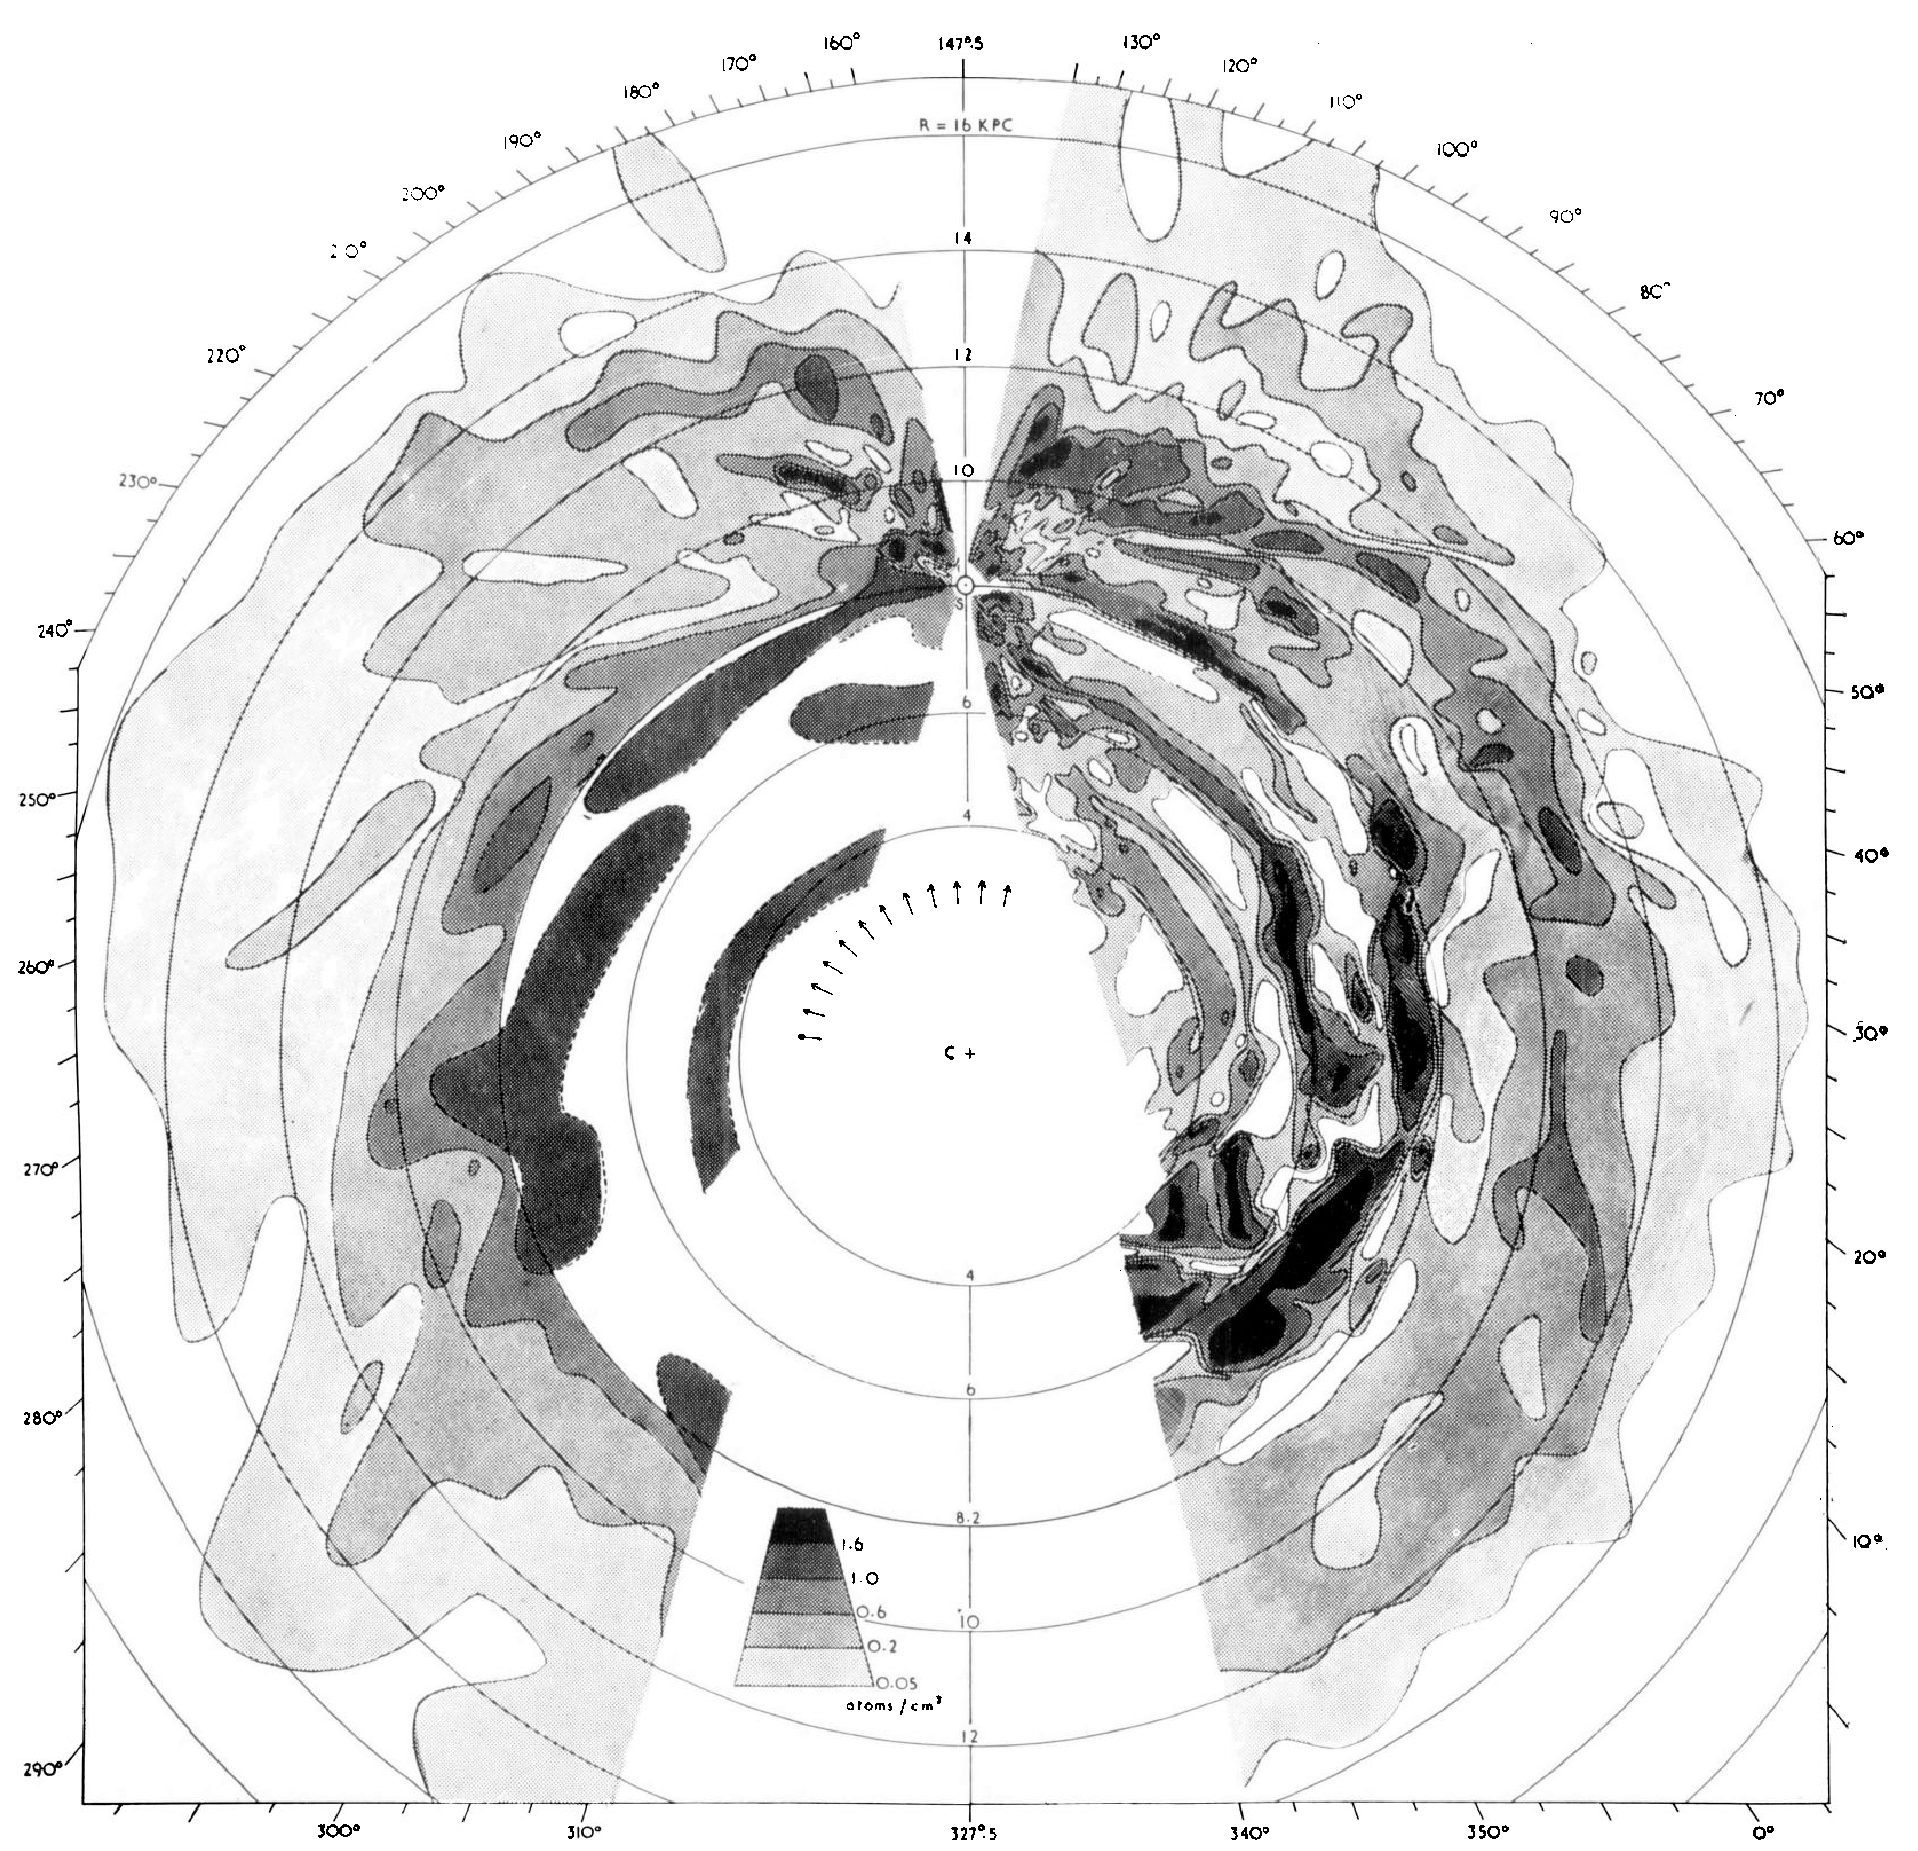
\includegraphics[width=\textwidth, angle=180]{./images/original_map.png}%
    \end{column}%
    \begin{column}{0.47\textwidth}%
      \begin{description}[Messung]
        \item[1958] Veröffentlichung der ersten \enquote{Karte} der Milchstraße
        \item[Autoren] J. H. Oort, F. J. Kerr und G. Westerhout
        \item[Messung] \SI{7.5}{\meter}-Teleskop (Leiden) \&  \SI{11}{\meter}-Teleskop (Sidney)
      \end{description}

      \begin{center}
      \parbox{0.85\linewidth}{\enquote{The \SI{21}{\centi\meter} oberservations brought about a revolution in the study of galactic structure}\cite{oort}} 
      \end{center}
    \end{column}%
  \end{columns}
\end{frame}
